\newcommand{\hlme}[1]{{\color{red}\bf #1}}

\author[Juan Cruz-Martinez]{}
\institute{University of Milan}

\subsection{Back to the future}

\begin{frame}{How can future-proof the methodology}{Do we trust our errorbands?}

    \small
    The smaller error bands in the NNPDF4.0 fits are driven both by the increased amount of data and the
    improved methodology.
    But there are still kin. regions not covered by data!

    \begin{columns}
        \column{0.6\linewidth}
        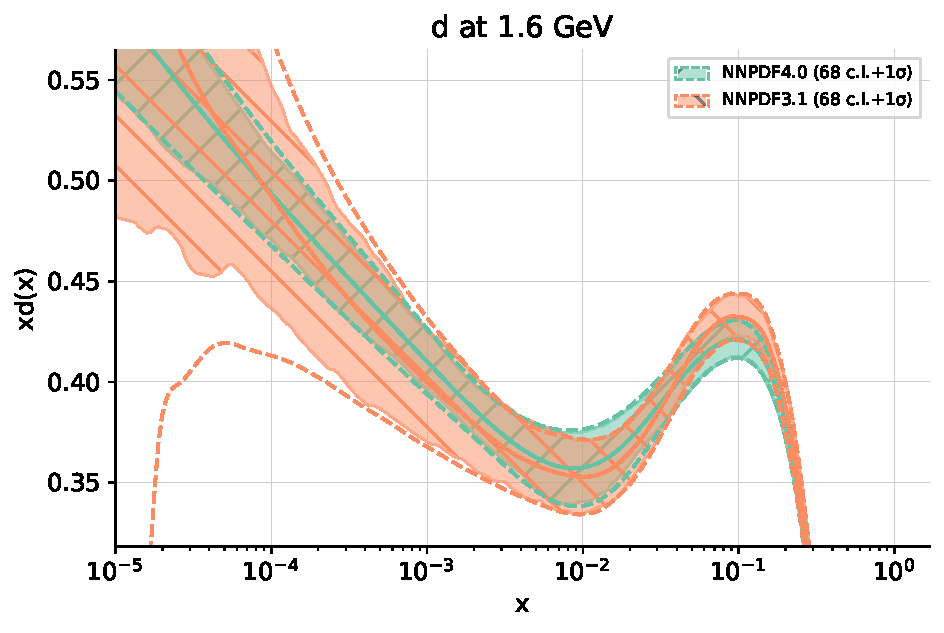
\includegraphics[width=1.0\textwidth]{juan_future_hyperopt/dquark.pdf}

        \column{0.4\linewidth} \vspace{-2.3cm} {

            Ideally: design an experiment for the regions not covered by fitted-data!

            \vspace{0.3cm}

            Problem: we want the results before 2050...

        }
    \end{columns}

    \vspace{-0.3cm}

    \begin{columns}
        \column{0.7\linewidth}
        Solution: chronologically ordered subsets of data to test unseen regions, we named this ``future tests``.

        \column{0.3\linewidth}
        \vspace{-1.9cm}
        \begin{figure}
            \captionsetup{format=smol}
            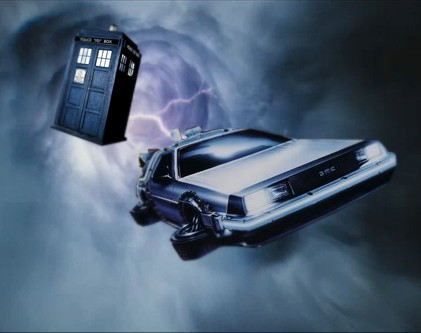
\includegraphics[width=0.7\textwidth]{juan_future_hyperopt/tardisdelorean.jpg}
            \caption{\tiny Other valid and certified future-testing methods}
        \end{figure}
    \end{columns}



\end{frame}


\begin{frame}{Future tests}{for more information see arxiv:21XX}

    \begin{columns}
        \column{0.60\linewidth}
        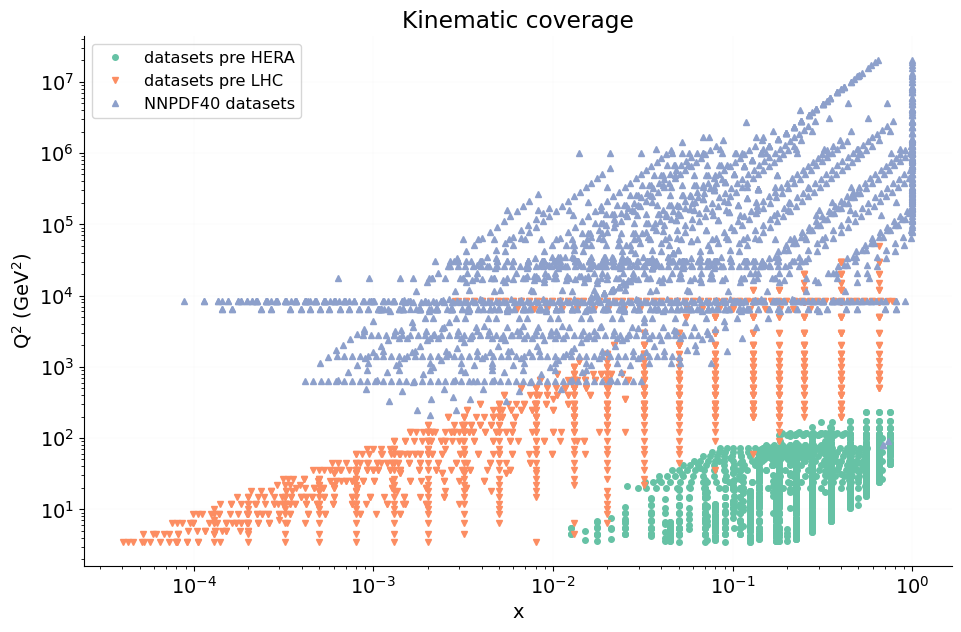
\includegraphics[width=\textwidth, height=0.8\textheight]{juan_future_hyperopt/kincov.png}
        \column{0.46\linewidth}
        \vspace{-0.9cm}
        \only<1>{
            \begin{table}
                \tiny
                \centering
                \caption*{\scriptsize $\chi^{2}/N$ (only exp. covmat)}
                \begin{tabular}{c | c c c} \toprule
                    (dataset) & NNPDF4.0 & pre-LHC & pre-Hera  \\ \midrule
                    pre-HERA  & 1.09 & 1.01 & 0.90 \\
                    pre-LHC   & 1.21 & 1.20 & \hlme{23.1} \\
                    NNPDF4.0  & 1.29 & \hlme{3.30} & \hlme{23.1} \\
                    \bottomrule
                \end{tabular}
            \end{table}
        }
        \only<2>{
            \begin{table}
                \tiny
                \centering
                \caption*{\scriptsize $\chi^{2}/N$ (exp. and PDF covmat)}
                \begin{tabular}{c | c c c} \toprule
                    (dataset) & NNPDF4.0 & pre-LHC & pre-Hera  \\ \midrule
                    pre-HERA  &  & & 0.86 \\
                    pre-LHC   &  & 1.17 & \hlme{1.22} \\
                    NNPDF4.0  & 1.12 & \hlme{1.30} & \hlme{1.38} \\
                    \bottomrule
                \end{tabular}
            \end{table}
        }


        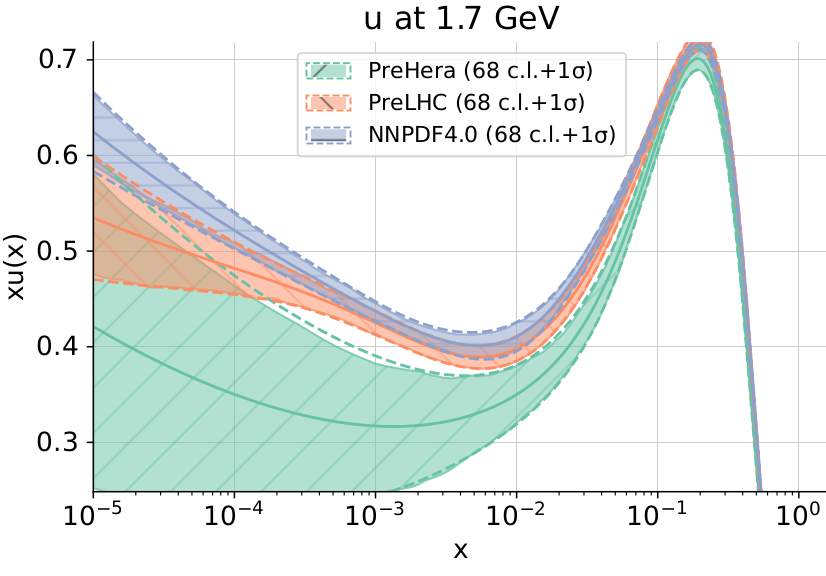
\includegraphics[width=1.0\textwidth]{juan_future_hyperopt/diffu}

    \end{columns}
\end{frame}
